%!TEX root = ./main.tex
%!TEX encoding = UTF-8 Unicode
\chapter{Installation de \harmless, génération d'un simulateur}
\section{Chaîne de développement}
La chaîne de développement autour du langage de description d'architecture \harmless\ est composé d'un certain nombre d'outils qui interagissent suivant le schema \ref{fig:devTool}.
\begin{figure}		%% Small Example
  \begin{center}
    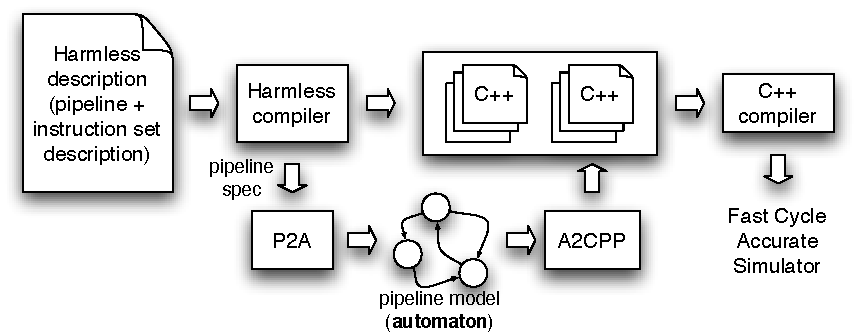
\includegraphics[width=0.8 \linewidth]{../common/images/devTools.pdf}
    \caption{Chaîne de développement.}
    \label{fig:devTool}
  \end{center}
\end{figure}

Ces outils sont:
\begin{itemize}
\item \gadl\ s'occupe de lire le fichier de description dans le langage \harmless. C'est le seul outil nécessaire si on souhaite générer un simulateur de jeu d'instruction (ISS);
\item p2a et a2cpp sont des outils qui sont utilisés pour la modélisation du pipeline, lors de la description de l'architecture interne. Un fichier de description du pipeline est généré par \gadl\ en fonction de la description, et celui-ci est le fichier d'entrée de p2a. Une fois l'automate généré par p2a, le deuxième outil a2cpp s'occupe de générer le code $C++$ associé à la modélisation du pipeline.
\end{itemize}

Nous nous intéressons dans une première approche qu'à l'utilisation de l'outil \gadl, car l'intégration avec les 2 autres outils est en cours de développement.

\section{Installation de \gadl\ à partir des sources}
\subsection{Compilation de \gadl}
le compilateur \gadl\ est entièrement écrit en utilisant le langage \emph{Galgas} qui est un compilateur de compilateur. \emph{Galgas} est écrit par Pierre Molinaro à l'IRCCyN et \gadl\ se synchronise toujours avec la version la plus à jour. Les sources, ainsi que les consignes pour l'installation de \emph{Galgas} sont disponibles sur \url{http://galgas.rts-software.org}.

Il y a dans l'archive des sources de gadl un certain nombre de dossiers commençant par \texttt{makefile\_} qui permettent de compiler \gadl\ pour différentes plate-forme (Linux, Mac OSX et MS Windows). Pour Linux par exemple:
\begin{verbatim}
$ cd makefile_unix
$ make gadl
\end{verbatim}
Par defaut, le makefile génère 2 exécutables \texttt{gadl} et \texttt{gadl\_debug}, ce dernier étant utilisé pour la mise au point (\texttt{gadl.exe} et \texttt{gadl\_debug.exe} sous MS Windows).

\emph{Note}: Pour une architecture 64 bits (Linux X86\_64 par exemple), il est nécessaire d'utiliser le makefile \texttt{makefile64}:
\begin{verbatim}
$ cd makefile_unix
$ make -f makefile64
\end{verbatim}
Dans ce cas, l'exécutable sera nommé \texttt{gadl64} et \texttt{gadl\_debug64}.

Pour plus de souplesse, il est conseillé de mettre le fichier généré dans le \texttt{PATH} par une copie dans \texttt{/usr/local/bin} par exemple:
\begin{verbatim}
$ sudo cp gadl /usr/local/bin
\end{verbatim}

L'effacement des fichiers générés se fait par la commande classique:
\begin{verbatim}
$ cd makefile_unix
$ make clean
\end{verbatim}

\subsection{Utilisation de templates}
\gadl\ utilise des templates pour la génération de code. C'est un ensemble de fichiers sources dans lesquels sont effectuées des opérations de remplacement de texte pour la génération es sources du simulateur. le dossier \texttt{templates} est utilisé par le compilateur gadl pour générer le code des simulateurs. 

Le dossier d'installation des templates peut être spécifié soit en ligne de commande lors de l'appel à gadl (\texttt{--templates=/path/to/templates}), soit dans une variable d'environnement (\texttt{GADL\_TEMPLATES}), par exemple dans un shell Bash:
\begin{verbatim}
$ export GADL_TEMPLATES=/path/to/templates
\end{verbatim}
Pour que la variable d'environnement soit conservée pour une autre session, il conseillé de mettre la commande précédente dans un script de démarrage du shell (\texttt{~/.profile} ou \texttt{~/.bashrc} par exemple)

\subsection{Editeur de description}
Un fichier de syntaxe fourni permet la coloration syntaxique pour l'éditeur Vim (ou gvim) disponible sur la plupart des systèmes d'exploitation. Il suffit de copier le fichier de syntaxe dans le dossier \texttt{~/.vim/syntax}. Il faut créer le dossier si celui-ci n'existe pas déjà.

Sous Mac Os X (10.4?), un projet XCode est fourni. Il permet de compiler directement gadl, mais aussi de construire une application (un bundle Mac OS X) permettant d'éditer les descriptions \harmless. Il embarque un éditeur de texte avec la coloration syntaxique, ainsi que le compilateur \gadl.


\section{Dépendances pour la génération d'un simulateur}

Le simulateur généré est écrit en $C++$ et doit pouvoir être utilisable directement, sans autre dépendance. Cependant, un certain nombre de dépendances peuvent être ajoutées, afin d'obtenir des possibilité supplémentaires:
\begin{description}
\item[python] Ceci permet de pouvoir utiliser le simulateur dans un script Python, et donc de ne pas recompiler le simulateur pour chaque nouveau scénario.
\item[libelf] Cette bibliothèque permet de lire les fichiers au format \emph{elf}, en plus des formats par défaut (Motorola SRecord et Intel Hex)
\end{description}

Cette section donne des indications sur la procédure pour installer ces dépendances.

\subsection{Utilisation du simulateur dans un environnement Python}
Le simulateur généré est en $C++$ et peut être utilisé dans un script Python (notamment). Pour permettre la compilation du \textit{wrapper} Python, il est nécessaire d'installer l'outil Swig\footnote{\url{http://www.swig.org/}}:
\begin{itemize}
\item sous Linux Ubuntu: les paquets \texttt{swig} et \texttt{python2.5-dev}. L'interpréteur Python 2.5 est installé par défaut (Ubuntu 8.04);
\item sous Mac Os X: tout est déjà inclus dans les outils de développement (sous 10.5);
\item sous MS Windows: le fonctionnalité n'est pas testée à ce jour.
\end{itemize}

\subsection{Bibiothèque de lecture des fichiers ELF}
\label{sec:elf}
Aucune bibliothèque supplémentaire n'est requise pour utiliser \gadl, le simulateur générer pourra alors lire les formats de fichiers:
\begin{itemize}
\item Motorola SRecord (SREC)\footnote{\url{http://en.wikipedia.org/wiki/SREC_(file_format)}};
\item Intel Hex\footnote{\url{http://en.wikipedia.org/wiki/Intel_HEX}};
\end{itemize}
Pour rajouter le support des fichiers au format ELF\footnote{\url{http://en.wikipedia.org/wiki/Executable_and_Linkable_Format}}, il faut rajouter une bibliothèque \texttt{libelf} supplémentaire. Ce dernier format présente l'énorme avantage d'encapsuler, en plus du code exécutable, les symboles des variable globales et des fonctions notamment. 

Attention toutefois, \gadl\ n'est pas compatible avec la bibliothèque \texttt{libelf} qui se trouve généralement sur les distributions Linux (Ubuntu notamment). En effet, la bibliothèque est liée au simulateur généré par \gadl\, et il n'est pas envisageable d'imposer que le code générer soit sous une licence compatible avec la GNU GPL\footnote{\url{http://fr.wikipedia.org/wiki/Licence\_publique\_generale\_GNU}}. Nous utilisons donc une bibliothèque sous licence GNU LGPL\footnote{\url{http://fr.wikipedia.org/wiki/Licence\_publique\_generale\_limitee\_GNU}} qui n'impose rien sur le code du simulateur généré. La bibliothèque \texttt{libelf} se trouve sur \url{http://www.mr511.de/software/english.html}. Pour l'installer:
\begin{verbatim}
$ ./configure
$ make
$ sudo make install
\end{verbatim}
Il n'est pas forcément souhaitable de faire l'installation de la bibliothèque sous Linux, celle-ci pouvant entrer en conflit avec d'autres présente. Dans ce cas, une utilisation en locale est préférable.

\emph{Note}: Par défaut, le simulateur généré est en 64 bits (\emph{flag} de compilation \texttt{-m64}), ce qui donne de bien meilleurs performances de simulation. Dans ce cas, la bibliothèque libelf doit supporter elle aussi le 64 bits:
\begin{verbatim}
$ ./configure
$ make CFLAGS=-m64 LDFLAGS=-m64
$ sudo make install
\end{verbatim}
Pour rester en 32 bits, il faudra alors modifier le fichier \texttt{Makefile} pour enlever le paramètre \texttt{-m64}.

\section{Génération d'un simulateur}
La génération du simulateur se fait à partir du fichier principal dans le cas d'une description répartie sur plusieurs fichiers (voir section \ref{sec:plusieursFichiers}).

L'appel à \gadl\ se fait en ligne de commande. Plusieurs options sont disponibles:
\begin{verbatim}
$ gadl --help
Compiled in 32 bits mode.
Usage : gadl [--help] [--version] [--lexical-analysis-only] [--parse-only] [-v] 
[--verbose] [--log-file-read] [--no-file-generation] [--Werror] 
[--detailled-error-messages] [-f] [--message-if-no-format] [-b] [--no-behavior] 
[-c] [--no-check] [-a] [--no-deasm] [-s] [--speed] [-t] [--warn-trunc] 
[--max-errorss=number] [--max-warningss=number] [--model=string] 
[--templates=string] file...
Options:
 --help               Display help information
 --version            Display version
 --lexical-analysis-only
                      Perform only lexical analysis on input files
 --parse-only         Parse only input files
 -v,--verbose         Verbose Output
 --log-file-read      Log every file read
 --no-file-generation Do not generate any file
 --Werror             Treat warnings as errors
 --detailled-error-messages
                      Print detailled error messages
 -f,--message-if-no-format
                      get a message when an instruction signature found in a behavior or a syntax part have no corresponding format.
 -b,--no-behavior     does not take into account instruction behavior part. It is not possible to generate an instruction set simulator (ISS)
 -c,--no-check        Remove time consuming checks: orthogonality of instruction set.
 -a,--no-deasm        does not take into account instruction syntax part. It is not possible to generate a dissassembler
 -s,--speed           speed option. May be more difficult to debug. Inline component methods.
 -t,--warn-trunc      Warn if the result of an expression may be truncated
 --max-errors=number (default value : 0)
                      Stop after the given number of errors has been reached (by default: 100)
 --max-warnings=number (default value : 0)
                      Stop after the given number of warnings has been reached (by default: 100)
 --model=string       model name that will be generated. By default, all the model defined in the description file are generated.
 --templates=string   Template directory
Handled extension:
 .hadl                a gadl file that can be parsed with an LL1 grammar
\end{verbatim}

Pour chaque modèle décrit dans la description (voir section \ref{sec:plusieursModeles}), un dossier est créé, contenant le code source du simulateur principalement. Soit par exemple le fichier de description \texttt{avr.hadl} (contenu dans les sources) qui contient le modèle \texttt{AT90CAN128}. La commande suivante
\begin{verbatim}
$ gadl ./avr.hadl
\end{verbatim}
provoque la création du répertoire \texttt{./AT90CAN128} qui contient tous les sources du simulateur. Les fichiers les plus importants sont:
\begin{verbatim}
Makefile           #le fichier de génération du simulateur (requiert GNU Make)
arch.h             #classe principale du simulateur (arch)
arch.i             #fichier pour l'interface C++/Python (pour Swig)
format_all.dot     #fichiers de description de l'arbre des formats (graphViz)
instConstruct.cpp  #constructeur des instructions (gros fichier)
instDecoder.cpp    #décodage des instructions (relié à 'format')
instExec.cpp       #Code exécuté par les instructions (relié à 'behavior')
instMnemo.cpp      #Mnémonique des instructions (relié à 'syntax')
instruction.h      #la définition des classes instructions
instruction.log    #information de mise au point généré par la syntaxe.
main.cpp           #scenario simple en C (non utilisé en Python)
storage.h          #modèle mémoire
types.h            #les différents types de données.
\end{verbatim}
\subsection{Paramètres de compilation}
\label{sec:cflags}
Lors de la compilation d'un simulateur, certains drapeaux peuvent être utilisés pour modifier le comportement du simulateur. 
Les principaux paramètres de compilations (CFLAGS dans le \emph{Makefile}) sont:
\begin{description}
\item[HOST\_IS\_LITTLE\_ENDIAN] L'hôte est \emph{little endian}. Cette information est utilisée par le module \emph{storage}.
\item[HOST\_IS\_BIG\_ENDIAN] L'hôte est \emph{big endian}. Cette information est utilisée par le module \emph{storage}.
\item[USE\_INTERACTIVE\_SIMULATION] Cette option est \emph{requise} pour l'utilisation des points d'arrêts (\emph{breakpoints}). Cette option ralentit légèrement la vitesse de simulation.
\item[INST\_DECODER\_CACHE\_STATS] Cette option permet d'enregistrer les information sur l'utilisation de la mémoire cache de décodage (nombre d'accès, ratio hit/miss). Cette option ralentit légèrement la vitesse de simulation.
\item[GADL\_NO\_ACTION] Cette option accélère notablement la vitesse de simulation. Les \emph{actions} sont utilisées pour associer l'exécution d'une routine lors d'un accès à la mémoire (en lecture, écriture ou exécution). Les actions sont utilisées notamment par les points d'arrêts!
\item[DEBUG\_MNEMO] Utilisé pour la mise au point du désassembleur. Lors de l'affichage du mnémonique, le nom interne de l'instruction est aussi affiché.
\item[DEBUG\_STORAGE\_ACCESS] Utilisé pour la mise au point. Chaque accès à la mémoire (lecture/écriture) est affiché sur la sortie standard. Cette option ralentit la vitesse de simulation.
\item[DO\_NOT\_USE\_INTERNAL\_INSTRUCTION\_CACHE] Utilisé pour la mise au point (et encore :-/). Permet de ne pas utiliser le cache d'instruction interne (lié au décodeur). Les performances sont réduites.
\item[DEBUG\_STORAGE\_ADDRESS\_RANGE] Utilisé pour la mise au point. Cette option permet de valider que chaque accès mémoire se situe dans une plage correcte. Cette option ralentit légèrement la vitesse de simulation
\end{description}

Un \emph{Makefile} permet de générer un exécutable et une bibliothèque utilisable sous forme de module à l'aide du langage Python. Il est nécessaire de modifier les paramètres du Makefile suivant la cible choisie (voir le fichier Makefile documenté). Les principales cibles sont:
\begin{description}
\item[make standalone] compilation du simulateur en mode \emph{standalone}, le scénario de simulation est contenu dans le fichier \texttt{main.cpp};
\item[make python] compilation du simulateur sous la forme d'une bibliothèque, utilisable depuis l'environnement \emph{Python}, voir \ref{sec:python};
\item[make] compilation à la fois du simulateur en mode \emph{standalone} et sous le forme de bibliothèque \emph{Python};
\item[make clean] effacement des fichiers binaires générés.
\end{description}


\section{Utilisation du simulateur}
les principales commandes pour la simulation sont disponible en C (en précisant le scénario de simulation directement dans le fichier \texttt{main.c}) ou en Python, si on utilise le wrapper Python (à l'aide de l'outil Swig).

L'objet ($C++$) principal est \texttt{arch} qui permet de créer une instance du simulateur.

\subsection{Observation du système}

\paragraph{\texttt{void decoderStats()}}
La méthode affiche les informations sur le décodeur (en fait sur le cache interne). Cette option n'est valable que si le cache de décodage est utilisé (pas d'option \texttt{DO\_NOT\_USE\_INTERNAL\_INSTRUCTION\_CACHE}) et que les statistiques sont autorisées (\texttt{INST\_DECODER\_CACHE\_STATS}), voir section \ref{sec:cflags}:
\begin{verbatim}
Internal decoder instruction cache Ratio
    12128 accesses.
    Miss : 1217
    Hit : 10911
    Hit Ratio : 0.899654
    cache contains : 524 instructions
    (capacity is 1024 instructions)
    cache use ratio : 0.511719
\end{verbatim}

\paragraph{\texttt{unsigned int const getNBCycles()}} Retourne le nombre de cycles depuis le début de la simulation. Cette variable n'est pas actualisée dans le cas de l'utilisation en mode ISS (simulation de jeu d'instruction).
\paragraph{\texttt{unsigned int const getNBInstructions()}} Retourne le nombre d'instructions utilisées depuis le début de la simulation.
\paragraph{\texttt{string disassemble(const unsigned int ipStart, const int nbInst, bool verbose)}} Permet le désassemblage du code à partir de l'adresse \texttt{ipStart}, pour \texttt{nbInst} instructions. Si verbose est à \texttt{true}, l'adresse de décodage ainsi que le code binaire de l'instruction sont également affichés.

\subsection{Execution}
\paragraph{\texttt{void reset()}}
Cette méthode se contente de réinitialiser le compteur programme pour l'instant.

\paragraph{\texttt{void execInst(const unsigned int nb)}} Permet d'exécuter \emph{au plus} \texttt{nb} instructions, que ce soit en mode CAS (Cycle Accurate Simulation) ou ISS (Instruciton Set Simulation). Si des points d'arrêts sont utilisés, l'exécution peut s'arrêter avant.

\paragraph{\texttt{void runUntil(const unsigned int addr, const unsigned int max)}} Permet de lancer la simulation jusqu'à ce que le compteur programme atteigne la valeur \texttt{addr}. La simulation execute \emph{au plus} \texttt{max} instructions. L'implémentation se fait en comparant après chaque instruction \texttt{addr} avec le compteur programme. Si les points d'arrêts sont disponible, il est plus efficace de les utiliser (pas de tests).

\paragraph{\texttt{bool readCodeFile(const char *filename, const bool verbose = false)}} Permet de lire un fichier binaire, et de le mettre en mémoire. Le fichier doit être dans un des formats reconnus (SRecord, Intel Hex ou .elf, voir section \ref{sec:elf}). Si aucun format ne correspond, une erreur est envoyée sur \texttt{stderr}. Uniquement les zones mémoires marquées \texttt{program} peuvent recevoir du code, dans la description de la mémoire (voir section \ref{sec:mem_program}).

\subsubsection{Points d'arrêts}
L'utilisation des points d'arrêts requière les \emph{actions} (exécution d'une routine C lors d'un accès en mémoire en lecture, écriture ou exécution). De plus il est indispensable de valider l'option permettant d'arrêter la simulation, soit les paramètres de compilation: \texttt{USE\_INTERACTIVE\_SIMULATION} et ne pas utiliser \texttt{GADL\_NO\_ACTION}, voir la section \ref{sec:cflags}.
\paragraph{\texttt{void addBreakpoint(const unsigned int addr)}} Ajoute un point d'arrêt à une adresse du code programme. Un message d'erreur est affiché sur \texttt{stderr} si un point d'arrêt est déjà présent.
\paragraph{\texttt{void addBreakpoint(const char *symbolName)}} Ajoute un point d'arrêt. Un symbole de fonction est utilisé à la place d'une adresse mémoire. Actuellement, les symboles sont extraits uniquement à partir d'un fichier au format .elf (voir section \ref{sec:elf}). Cette méthode s'appuie sur la précédente.
\paragraph{\texttt{void removeAllBreakpoints()}} Supprime tous les points d'arrêt.
\paragraph{\texttt{void removeBreakpoint(const unsigned int addr)}} Supprime le point d'arrêt à l'adresse spécifiée. Un message d'erreur est affiché sur \texttt{stderr} s'il n'y a pas de point d'arrêt à cette adresse.
\paragraph{\texttt{void removeBreakpoint(const char *symbolName)}} Supprime un point d'arrêt. Un symbole de fonction est utilisé à la place d'une adresse mémoire. Actuellement, les symboles sont extraits uniquement à partir d'un fichier au format .elf (voir section \ref{sec:elf}). Cette méthode s'appuie sur la précédente.

\paragraph{\texttt{storage * getProgramChunk(const unsigned int address)}} Permet d'obtenir l'objet mémoire correspondant à une adresse. Ceci permet ensuite de lire/écrire des données en mémoire (voir le fichier généré \texttt{storage.h} pour plus de détails).
\paragraph{\texttt{void setProgramCounter(u32 val)}} Permet de définir la valeur du compteur programme (indépendamment du nom utilisé dans l'architecture (IP, PC, ..)
\paragraph{\texttt{u32 programCounter()}} Permet d'obtenir la valeur du compteur programme (indépendamment du nom utilisé dans l'architecture (IP, PC, ..)

\subsection{Utilisation de symboles}
L'utilisation de symboles est possible à la place d'adresses mémoire uniquement pour les fichiers au format .elf (voir section \ref{sec:elf}).

\paragraph{\texttt{bool getSymbolObjectAddress(const char *symbolName, u32 \&v\_addr, u32 \&size)}} Cherche l'adresse correspondant à un symbole. Retourne \texttt{true} si le symbole est trouvé et actualise la taille (\texttt{size}) et l'adresse \emph{virtuelle}.
\paragraph{\texttt{bool getFunctionName(const char *symbolName, u32 \&v\_addr)}} Cherche l'adresse correspondant à une fonction. Retourne \texttt{true} si le symbole est trouvé et actualise l'adresse \emph{virtuelle}.
\paragraph{\texttt{u32 getPhysicalAddress(const u32 v\_addr, bool \&found)}}  Permet d'obtenir l'adresse physique, à partir de l'adresse virtuelle. \texttt{found} est mis à \texttt{false} si la valeur est impossible.

\subsection{Utilisation de Python}
\label{sec:python}
Le principal intérêt d'utiliser Python pour exécuter des scénarios vient du fait qu'il est inutile de recompiler le simulateur pour chaque nouveau scenario. Lors de la compilation, un wrapper est générer avec swig, et un module python est construit. Dans Python, il est alors possible d'appeler toutes les méthodes C définies dans la première partie de cette section. 
Considérons par exemple le simulateur de l'AVR qui est fourni dans les exemples. Le modèle s'appelle AT90CAN128, ce qui correspond au nom du module à appeler. Le script suivant permet de calculer le nombre d'instructions entre 2 accès à la fonction \texttt{function\_of\_task\_startTask}, ce 10 fois de suite:
\lstset{language=Python}
\begin{lstlisting}
#!/usr/bin/python
from AT90CAN128 import arch

f=arch()
f.readCodeFile("../trampoline.elf")
f.addBreakpoint("function_of_task_startTask")
i = 0
nbInst = 0
f.printRegs()
while i < 10:
    f.execInst(10000000) #run until breakpoint
    print f.getNBInstructions() - nbInst,  " insts between 2 breakpoints"
    nbInst = f.getNBInstructions()
    i = i+1
f.printRegs()
f.decoderStats()
\end{lstlisting}
\lstset{language=Harmless}
